\documentclass[a4paper]{article}

\usepackage[utf8]{inputenc}
\usepackage{polski}
\usepackage[polish]{babel}
\usepackage[margin=1in]{geometry}
\usepackage{lmodern}
\usepackage{tabularx}
\usepackage{graphicx}
\newcounter{counter}
\newcommand\rownumber{\stepcounter{counter}\arabic{counter}}

\title{\textbf{Podsumowanie prac z projektu WDS - kwiecień 2015}}
\author{Marcin Ochman - 200546}
\date{}
\begin{document}


\begin{titlepage}
\begin{center}

 \newcommand{\HRule}{\rule{\linewidth}{0.5mm}}
%\includegraphics[width=0.15\textwidth]{./logo}~\\[1cm]

\textsc{\Large Projekt z Wizualizacji danych sensorycznych}\\[1cm]

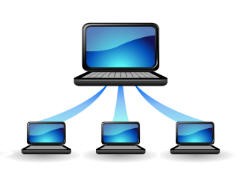
\includegraphics{network_icon}


\HRule \\[0.4cm]
{ \huge \bfseries \textit{Computer Monitor} - monitorowanie komputerów poprzez sieć.\\[0.4cm] }

{\huge \underline{\textit{Raport postępu prac }}}\\[0.5cm]


\LARGE 23.04.2015
\HRule \\[1.5cm]


\noindent
\begin{minipage}[t]{0.4\textwidth}
\begin{flushleft} \large
\emph{Autor:}\\
Marcin \textsc{Ochman}
\end{flushleft}
\end{minipage}%
\begin{minipage}[t]{0.4\textwidth}
\begin{flushright} \large
\emph{Prowadzący} \\
Dr inż. Bogdan \textsc{Kreczmer}
\end{flushright}
\end{minipage}


\end{center}
\end{titlepage}

\newpage

\tableofcontents
\listoffigures
\listoftables

\newpage

	\section{Założenia projektowe}
		Celem projektu jest napisanie aplikacji \textit{,,Computer Monitor''} przeznaczoną na komputery osobiste, która:
	\begin{itemize}
		\item pozwala na monitorowanie pracy komputera(ów), z którym(i) komputer jest połączony poprzez sieć
		\item pracuje w różnych trybach:
		\begin{itemize}
			\item tryb wizualizacji
			\item tryb raportowania
			\item połączenie dwóch poprzednich trybów
		\end{itemize}
		\item potrafi zapamiętać ustawienia użytkownika, w tym m.in. tryb działania aplikacji, układy okien, ustawienia wykresów itp.
		\item posiada przejrzysty, intuicyjny, atrakcyjny oraz konfigurowalny interfejs użytkownika rozumiany w następujący sposób:
		\begin{itemize}
			\item będą wyraźnie zaznaczone różne kategorie monitorowanych wielkości np. procesor, karta graficzna, pamięć \uppercase{ram}
			\item zaimplementowanie animacji
			\item dostosowywanie wykresów np. skala osi czasu
			 
		\end{itemize}
		\item pomimo realizowanej komunikacji poprzez sieć oraz innych zadań, jest wysoce 
		interaktywna
		\item docelową platformą jest system Linux, jednak zostaną poczynione wszelkie starania, aby aplikacja działała również na systemach Windows
	\end{itemize}
	
	\section{Opis poszczególnych trybów pracy}
	Poniżej zostały opisane poszczególne tryby pracy aplikacji.
	
	\subsection{Tryb wizualizacji}
		W tym trybie program prezentuje dane, które są pobierane poprzez sieć. Pozwala na śledzenie wartości poszczególnych wielkości opisujących stan komputera oraz prezentowanie danych na wykresach (zależności czasowe, zużycie zasobów komputera np. w formie wykresu kołowego) oraz diagramach/ilustracjach (monitorowanie i alarmowanie poprawności funkcjonowania systemu). Progi alarmowe można również zdefiniować samodzielnie. Dodatkowo będzie możliwość zapisywania raportów zawierających dane zdobyte w trakcie monitorowania.
	
	\subsection{Tryb raportowania}
		Program działający w trybie raportowania ma za zadanie śledzenie pracy komputera oraz wysyłanie zebranych informacji poprzez sieć. Użytkownik ma możliwość wyboru danych, które zostaną wysłane. Aplikacja będzie działać w systemowym zasobniku.
	
	\subsection{Tryb łączony}
		Jest to połączenie dwóch poprzednich trybów. Pozwala na jednoczesne wizualizowanie aktualnego stanu komputera, na którym została uruchomiona aplikacja oraz wysyłanie zebranych informacji poprzez sieć. Dwa ostatnie tryby zostały wyodrębnione ze względu na umożliwienie optymalizacji zasobów zajmowanych przez aplikację.
	


\section{Wstęp raportu}

W ciągu miesiąca tj. 18.03-23.04 zostało wykonanych wiele prac nad aplikacją. W tym dokumencie opisano wykonane i przewidywane na następny miesiąc zadania oraz komentarz autora na temat postępów prac nad aplikacją.

\section{Lista wykonanych zadań w projekcie}

W poniższej tabeli zostały zebrane zadania, które udało się zrealizować do dnia 23.04.2015r.

\begin{table}[h]
\centering
\begin{tabularx}{0.7\linewidth}{ |c|X| }
			\hline 
			\rownumber & Opracowano architekturę aplikacji - użyte biblioteki oraz 
						 klasy do napisania\\ \hline
			\rownumber & Utworzono strukturę katalogów aplikacji \\ \hline
			\rownumber & Aplikacja buduje się przy pomocy wieloplatformowego narzędzia 
						 \textit{CMake} - napisanie plików potrzebnych do poprawnej kompilacji \\ \hline
			\rownumber & Rozpoczęto pracę nad biblioteką \textit{SystemMonitoringLib} \\ \hline
			\rownumber & Rozpoczęto pracę nad interfejsem użytkownika \\ \hline
			\rownumber & Rozpoczęta pracę nad komunikacją pomiędzy biblioteką \textit{SystemMonitoringLib} oraz interfejsem użytkownika \\ \hline
	\end{tabularx}
	\caption{Tabela prac nad aplikacją}
\end{table}

\section{Szczegółowy opis wykonanych zadań}

\subsection{Opracowanie architektury aplikacji}
Program będzie opierać się na bibliotekach \textit{Qt5} i \textit{QCustomPlot}, które posłużą do prezentacji danych oraz autorskiej biblioteki, która została opisane w następnych punktach - \textit{SystemMonitoringLib}. Biblioteki monitorujące będą komunikować się z warstwą prezentacji za pomocą odpowiedniej klasy pośredniczącej. Diagram budowy aplikacji został przedstawiony na rysunku \ref{diagram_budowy_aplikacji}, a diagramy klas zostały przedstawione na rysunkach \ref{diagram_klas_system_monitoring} oraz \ref{diagram_klas_gui}, a diagram przypadków użycia na rysunku \ref{diagram_przypadkow_uzycia}.

\begin{figure}[h]
	\centering
	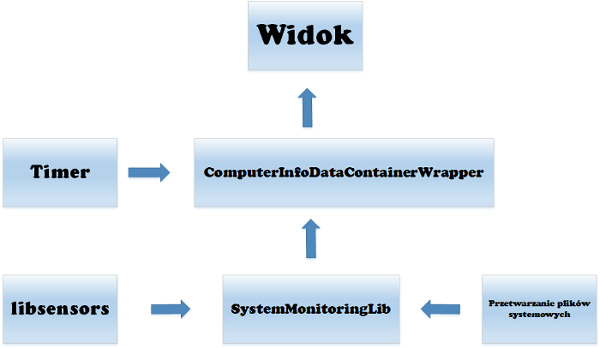
\includegraphics[width=\linewidth]{img/diagramBudowyAplikacji.png}
	\caption{Diagram budowy aplikacji}
	\label{diagram_budowy_aplikacji}
\end{figure}


\begin{figure}[h]
	\centering
	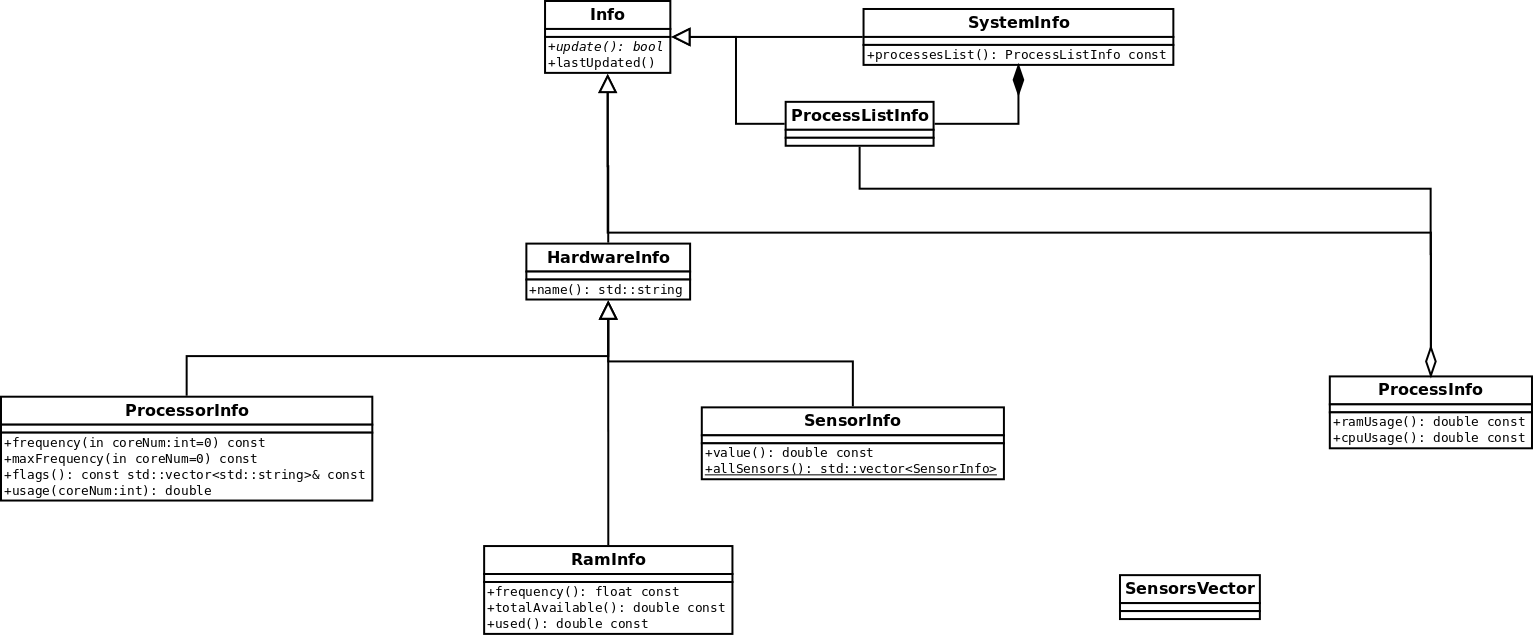
\includegraphics[width=0.75\paperheight, angle=90]{img/diagramKlas.png}
	\caption{Diagram UML stworzonych klas niezwiązanych z interfejsem użytkownika}
	\label{diagram_klas_system_monitoring}
\end{figure}

\begin{figure}[h]
	\centering
	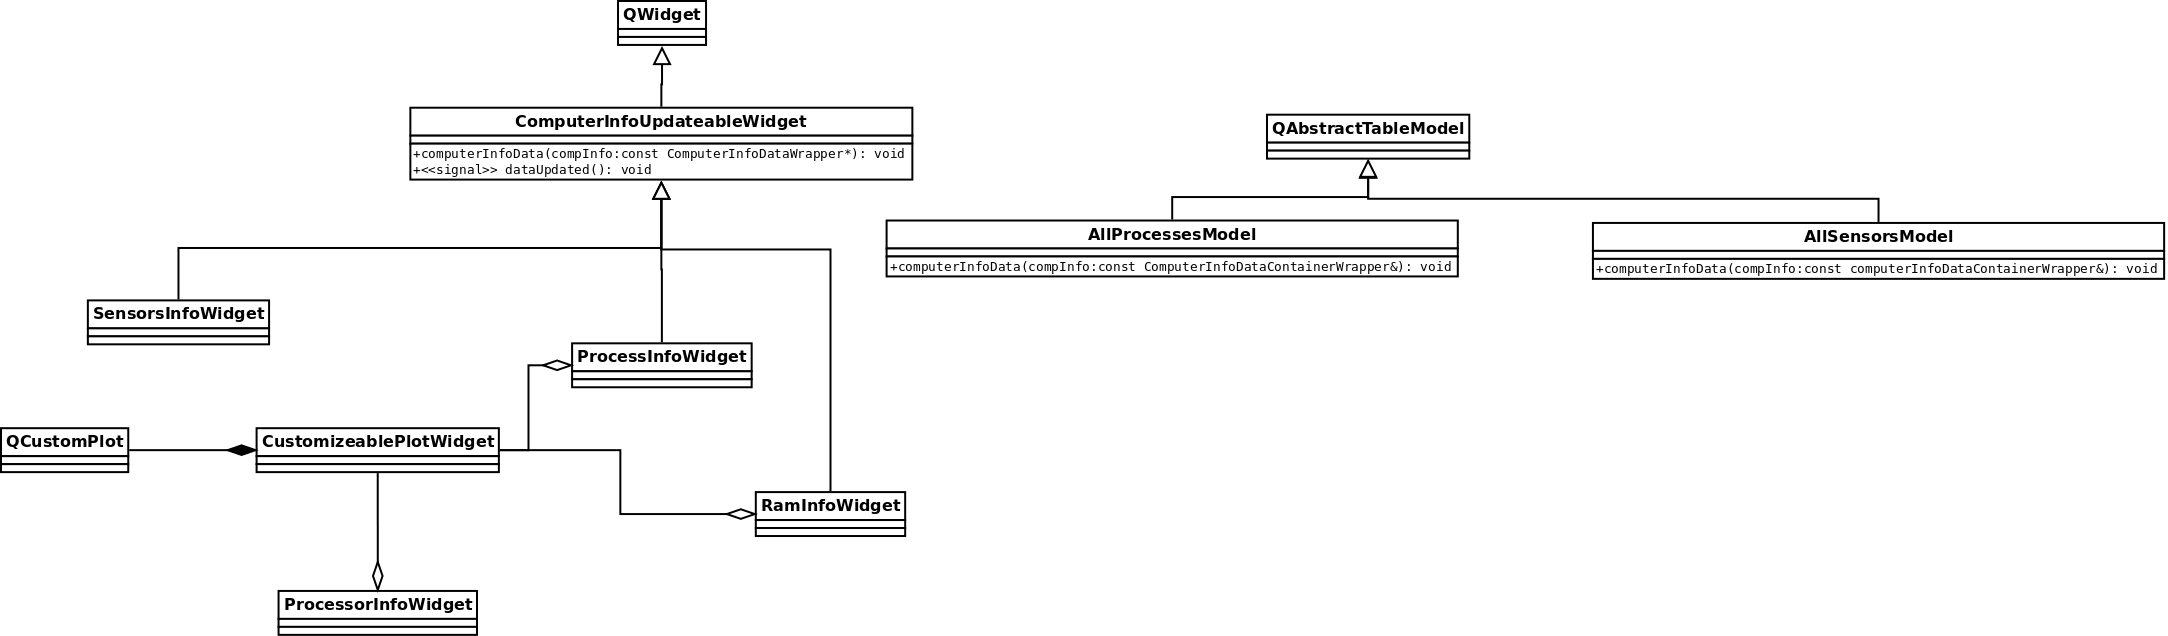
\includegraphics[width=0.75\paperheight, angle=90]{img/diagramKlasGui.png}
	\caption{Diagram UML klas związanych z interfejsem użytkownika}
	\label{diagram_klas_gui}
\end{figure}

\begin{figure}[h]
	\centering
	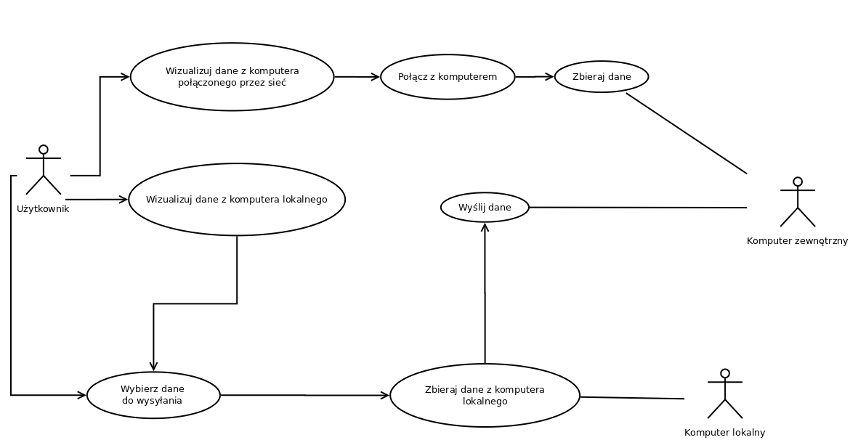
\includegraphics[width=0.75\paperheight, angle=90]{img/diagramPrzypadkowUzycia.png}
	\caption{Diagram przypadków użycia}
	\label{diagram_przypadkow_uzycia}
\end{figure}

\subsection{Stworzenie zalążka aplikacji}

Zalążek aplikacji wymagał kilku pomniejszych kroków do wykonania:
\begin{itemize}
	\item utworzenie struktury folderów projektu
	\item napisanie skryptów kompilujących i konsolidujących
\end{itemize}
Opis poszczególnych zadań znajduje się poniżej.

\subsubsection{Struktura folderów projektu}
W głównym folderze aplikacji znajdują się dwa foldery: \textit{doc} oraz \textit{prj}. Pierwszy zawiera wszelkie pliki przechowujące informacje o dokumentacji, a drugi zawiera kody źródłowe aplikacji. W folderze \textit{prj} można wyróżnić kilka folderów. Ich krótki opis zebrano w tabeli \ref{opis_folderow_prj}.

\begin{table}
\centering
\begin{tabularx}{0.7\linewidth}{|c|X|}
	\hline
	inc & przechowuje wszystkie pliki nagłówkowe, które nie należą do bibliotek \\ \hline
	src & zawiera pliki źródłowe, które nie należą do bibliotek \\ \hline
	lib & przechowuje pliki źródłowe oraz nagłówkowe bibliotek, każda biblioteka jest umieszczona 
		  w innym folderze. W każdym z folderów są pliki nagłówkowe oraz źródłowe \\ \hline
	ui & znajdują się w nim wszystkie pliki  programu QtDesigner \\ \hline
	rsrc  & zawiera zasoby aplikacji \\ \hline
\end{tabularx}
\caption{Opis poszczególnych folderów w katalogu \textit{prj/}}
\label{opis_folderow_prj}
\end{table}

\subsubsection{Proces kompilacji oraz opis narzędzia \textit{CMake}}
Program \textit{CMake} to wieloplatformowy system do budowania aplikacji. Dzięki niemu łatwe staje się
znajdowanie odpowiednich plików nagłówkowych oraz bibliotek oraz kompilacja na różnych platformach (m.in. Linux i Windows). Każdy folder zawiera w sobie plik \textit{CMakeLists.txt}, który definiuje w jaki sposób ma zachować się program budujący.Dzięki niemu, oszczędzono wiele czasu na kompilację oraz konsolidację programu używającego bibliotek \textit{Boost} oraz \textit{Qt5}. Najpierw budowane są biblioteki, a następnie cały program. Wszystko zostaje skonsolidowane. Istnieje również możliwość wygenerowania dokumentacji, wystarczy, że zbudujemy cel \textit{doc}.

\subsection{Biblioteka \textit{SystemMonitoringLib}}
Jest to biblioteka do monitorowania lokalnego komputera oraz wysyłania informacji przez sieć. Pozwala na pobieranie odczytów z czujników, informacji o procesorze takich jak częstotliwość taktowania poszczególnych rdzeni, zużycie procesora, o pamięci RAM (dostępna pamięć, zużycie) oraz informacje o poszczególnych procesach. Na komputerze z uruchominionym systemem \textit{Linux}, biblioteka do zbierania informacji o komputerze używa innej biblioteki - \textit{sensorslib} oraz przetwarze pliki m.in. \textit{/proc/stat/}, \textit{/proc/cpuinfo}

\subsection{Interfejs użytkownika}
Roczpoczęto prace nad wizualizowaniem danych  odczytanych z czujników dostępnych na płycie głównej.
W widoku tabelki mamy możliwość podglądania aktualnych wartości odczytanych wielkości. Zrzut ekranu przedstawiającego aktualny stan interfejsu użytkownika został pokazany na rysunku \ref{wygladAplikacji}.

\begin{figure}[h]
	\centering
	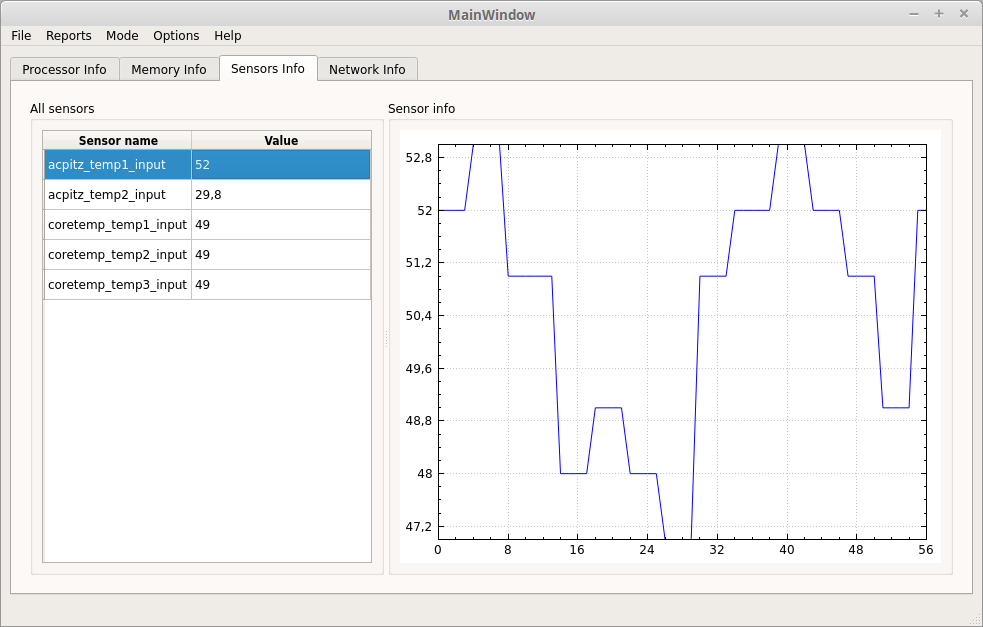
\includegraphics[width=\linewidth]{img/wygladAplikacji.png}
	\caption{Wygląd aplikacji \textit{ComputerMonitor}}
	\label{wygladAplikacji}
\end{figure}

\section{Opis zrealizowanych, planowanych i zaniechanych funkcjonalności}

Na dzień 23.04.2015 została zrealizowana funkcjonalność wizualizacji danych z czujników. Planowane funkcjonalności nie zmieniły się - są zgodne z tym co można znaleźć w założeniach projektu. Niestety ze względu na niedostateczną ilość czasu wersja na system \textit{Windows} została wstrzymana.

\section{Następne zadania do wykonania - aktualizacja planu pracy}
Ze względu na to, że niektóre zadania zostały wykonane ponad plan, a pewna część zadań z planu została nie zrealizowana należało zastosować poprawki w planie pracy nad aplikacją. Tabela \ref{tabela_harmonogram} przedstawia zaktualizowany plan pracy.
\begin{table}[h]
			\centering
			\begin{tabularx}{0.65\textwidth}{|c|X|}
				\hline
				Lp. & Opis \\ \hline
				1 & Stworzenie biblioteki, która pozwoli na pobieranie informacji o stanie komputera \\ \hline
				2. & Zaprogramowanie biblioteki służącej do komunikacji komputerów w siecie w celu wysyłania informacji zgromadzonych przez bibliotekę z pkt 1 \\ \hline
				3. & Zaprojektowanie oraz oprogramowanie interfejsu użytkownika \\ \hline
				4. & Połączenie pracy bibliotek z interfejsem użytkownika \\ \hline
			\end{tabularx}
			\caption{Tabela przedstawiająca kamienie milowe}
		\end{table}
\begin{table}[h]
			\centering
			\begin{tabularx}{\linewidth}{|c|c|c|X|}
				\hline
				Od & Do & Osiągnięty kamień milowy & Opis \\ \hline
				20.04 & 26.04 &  & Zapoznanie się z metodami programowania sieciowego i dostępnymi bibliotekami oraz  rozpoczęcie implementacji biblioteki sieciowej, Prace nad biblioteką monitorującą\\ \hline
				27.04 & 03.05 & 1 & Początki implementacji biblioteki sieciowej oraz finalizacja prac nad biblioteką monitorującą \\ \hline
				04.05 & 10.05 &  & Prace nad klasami do komunikacji sieciowej \\ \hline
				11.05 & 17.05 & 2  & Zakończenie prac nad komunikacją sieciową  \\ \hline
				18.05 & 24.05 &  & Dalsze projektowanie interfejsu użytkownika oraz jego implementacja \\ \hline
				25.03 & 31.03 & 3 & Implementacja interfejsu użytkownika oraz połączenie logiki programu z interfejsem \\ \hline
				01.06 & 07.06 & 4 & Ostateczne połączenie aplikacji graficznej z bibliotekami oraz początek testów aplikacji \\ \hline
				07.06 & 13.06 &  & Ostateczne testy aplikacji \\ \hline
			\end{tabularx}
			\caption{Tabela przedstawiająca uaktualniony harmonogram przyszyłych prac nad aplikacją}
			\label{tabela_harmonogram}
		\end{table}
Dla porównania umieściłem również stary harmonogram z zaznaczeniem, które podpunkty zostały do tej pory zakończone lub rozpoczęte. Przedstawia go tabela \ref{tabela_harmonogram_stary}.

		\begin{table}[h]
			\centering
			\begin{tabularx}{\linewidth}{|c|c|c|X|c|}
				\hline
				Od & Do & Osiągnięty kamień milowy & Opis & Status \\ \hline
				23.03 & 29.03 &  & Zaprojektowanie interfejsu biblioteki do monitorowania komputera & Ukończono  \\ \hline
				30.03 & 05.04 &  & Zapoznanie się z metodami dostępu do informacji o komputerze oraz rozpoczęcie implementacji powyższej biblioteki & Ukończono \\ \hline
				06.04 & 12.04 & 1 & Ukończenie biblioteki monitorującej komputer & W trakcie \\ \hline
				13.04 & 19.04 &   & Rozpoczęcie projektowania interfejsu biblioteki do komunikacji sieciowej & Rozpoczęto\\ \hline
				20.04 & 26.04 &  & Zapoznanie się z metodami programowania sieciowego i dostępnymi bibliotekami oraz  rozpoczęcie implementacji biblioteki sieciowej & --------- \\ \hline
				27.04 & 03.05 &  & Implementacja biblioteki sieciowej & --------- \\ \hline
				04.05 & 10.05 & 2 & Zakończenie prac nad biblioteką sieciową oraz rozpoczęcie projektowania interfejsu użytkownika & Rozpoczęto \\ \hline
				11.05 & 17.05 &    & Kontynuacja projektowania interfejsu użytkownika oraz jego implementacja & Rozpoczęto\\ \hline
				18.05 & 24.05 &  & Implementacja interfejsu użytkownika & Rozpoczęto\\ \hline
				25.03 & 31.03 & 3 & Implementacja interfejsu użytkownika oraz połączenie logiki programu z interfejsem & Rozpoczęto \\ \hline
				01.06 & 07.06 & 4 & Łączenie aplikacji graficznej z bibliotekami oraz początek testów aplikacji & Rozpoczęto \\ \hline
				07.06 & 13.06 &  & Ostateczne testy aplikacji & --------- \\ \hline
			\end{tabularx}
			\caption{Tabela przedstawiająca stary harmonogram ze statusem zadania}
			\label{tabela_harmonogram_stary}
		\end{table}

\section{Podsumowanie}
Ze względu na dużą liczbę innych projektów, prace nad aplikacją są lekko opóźnione - około tygodnia, jednak zostaną poczynione wszelkie starania aby do następnego terminu oddania prac wszystko zostało nadrobione. 
Pozytywną informacją jest fakt, że zostały już rozpoczęte prace nad interfejsem użytkownika, czego początkowy plan pracy nie uwzględniał.

\end{document}